% ============================================================================
% VII. v2 RESULTS: THE BOUNDARY TEST
% Design (PREREG_V2 Sec. 3, as merged at 1d8900c; THEORY Sec. 6.2):
%   both architectures run on the same test items, seeds, latency profile and
%   price; the architecture is the only thing that changes.
%   D*[COMMIT] = B9+;  D*[SPECULATIVE] = best on dev of {B9+, B10 (SPEC),
%   B11 (SPEC-theta)}, named at freeze.
%   Delta_C = D-bar(Ours-v2[C] - D*[C]);  Delta_S = D-bar(Ours-v2[S] - D*[S]).
%   P1: Delta_C > 0.   P2: Delta_C - Delta_S > 0 (paired interaction).
%   P3: TOST, -m3 < Delta_S < m3, m3 = 1/2 * delta_C,dev (fixed at freeze).
%   Boundary claim iff P1, P2 and both halves of P3 reject at one-sided
%   alpha = 0.025 (intersection-union test). Single claims: Holm across the
%   three (P3 at the larger of its two p-values).
% FROZEN VERSION (supersedes the lines above where they differ; PREREG_V2
%   FROZEN 2026-10-16, tag prereg-v2-frozen, code ddde67f):
%   D*[SPEC] = B9+ (d1_open), SPEC/B10 (d2_support); m3 = 0.016 fixed as
%   the smallest effect size of interest (the half-dev-effect rule was
%   degenerate because dev Delta_C < 0); H-REV (Delta_C < 0) added before
%   the freeze; Holm over {P1, P2, P3, H-REV} at one-sided 0.025.
%   Deviations D1-D3 and notes N1-N3 are logged in PREREG_V2 "Deviations".
% RESULTS (final; docs/research_v2/v2_test_results_final.{md,json}, commit
%   341d306; d1-only detail docs/research_v2/v2_test_results_d1.{md,json}):
%   STATUS RULE for every number below: d1_open = pre-registered
%   per-dataset analysis (unaffected by D3); d2_support and EVERY pooled
%   result = EXPLORATORY, because the judge that grades d2_support agreed
%   only moderately with the human labels (one annotator, 300 d2 dev
%   answers: gpt-6.1-sol 240/300, 80.0%, kappa 0.55; GPT-4o 244/300, 81.3%,
%   kappa 0.58). Describe the human check only in these words.
% Records: frozen-evaluator contrasts simulator/e3v2_phase_a/<ds>/contrasts_test.json
%   (in the confirmatory-run worktree); analysis analysis/v2_test_final.py.
% ============================================================================
\section{v2 Results: The Boundary Test}\label{sec:v2}

% ---- P-VII.1 -----------------------------------------------------------------
% PURPOSE: state the boundary test and why its three parts are needed
%   (Table~\ref{tab:predictions}).
% CLAIMS:
%   (a) The theory predicts a joint advantage when a dispatched retrieval is
%       committed (Prop. 4) and none beyond a belief-gated decomposed
%       prefetcher when it can be discarded (Prop. 4''). P1 tests the first,
%       P3 the second, and P2 tests that the change between them is caused
%       by the architecture, on the same items.
%   (b) WHY SPEC-THETA (B11) IS A REQUIRED RIVAL (Prop. 4''; outline note,
%       no citation needed): under speculation the joint controller can win
%       against "always prefetch" (B10) simply by not prefetching on turns
%       where the prefix already makes retrieval unlikely to be used, which
%       saves compute. That saving needs only the belief at the trigger and
%       fixed prices, so a decomposed controller can capture it: B11 does,
%       and the remaining joint advantage over B11 is a C1-sized term.
%       Without B11 in D*[SPECULATIVE], Delta_S would measure this
%       decomposable compute saving, not joint control. In simulation it is
%       0.013 to 0.015, larger than Delta_C (0.009 to 0.011), so P2 would be
%       predicted FALSE at every price and the conjunction could not pass at
%       any N [PRE2 Sec. 6.1; POW boundary_test].
%   (c) WHY THE MARGIN IS 1/2 delta_C: the earlier margin lambda_c(1+w)q is
%       not a valid bound (counterexample, Prop. 4'(3)), and at about 0.029 it
%       is roughly three times Delta_C, so P3 would follow from P2 almost for
%       free. Half the dev commit effect makes P3 say that speculation removes
%       at least half the commit advantage; the lower TOST side checks that
%       the joint speculative controller is not broken [THEORY Sec. 6.2].
% NUMBERS (dev-predicted, simulation, NOT results): 0.013-0.015;
%   0.009-0.011; 0.029 [PRE2 Sec. 6.1].
% CONTRADICTS FROZEN PREREG / FINAL RESULTS: (c) is obsolete -- the frozen
%   margin is m3 = 0.016, the smallest effect size of interest (the dev MDE
%   for Delta at the planned N), because 1/2 max(delta_C,dev, 0) = 0 on dev
%   (PRE2 Sec. 3.2). The simulation numbers in (b) are from the superseded
%   pre-dev planning simulation (PRE2 Sec. 6.2): dev reversed the sign of
%   Delta_C (pooled dev -0.0409, SE 0.0085; PRE2 Sec. 3.6), which is why
%   H-REV was added. On dev, D*[SPEC] for d2_support is SPEC (B10), which
%   ties SPEC-theta exactly (0.35795); for d1_open B9+ beats both
%   (0.3398 vs 0.3325) [PRE2 Sec. 3 "Rivals"; v2_predictions.json].
%   P-VII.1 must also introduce H-REV (PRE2 Sec. 3.3).
\todo{P-VII.1: the boundary test, its three parts and the intersection--union
decision rule; why \SPECth{} must be a rival and why the P3 margin is half the
commit effect.}

\subsection{Gatekeeping Checks}\label{sec:v2-gates}
% ---- P-VII.2 -----------------------------------------------------------------
% PURPOSE: report the gates that condition the main tests, in the order the
%   pre-registration lists them.
% NUMBERS (filled):
%   (a) Judge vs the one human labelling (300 d2 dev answers): gpt-6.1-sol
%       240/300 (80.0%, kappa 0.55), GPT-4o 244/300 (81.3%, kappa 0.58)
%       [simulator/judge_validation/v2_labeling/results/gate_report_v2.json].
%       One clause: because agreement is moderate, d2_support and pooled
%       accuracy results are reported as exploratory; d1_open uses alias
%       matching and needs no judge. Optional (d1_open, stratified
%       400-answer test subsample graded by both judges; log
%       test_logs/conf_d2_d1sub.log, labels_test.json): alias vs
%       gpt-6.1-sol 365/400 (kappa 0.82), alias vs GPT-4o 355/400 (kappa
%       0.77), judges 372/400 (kappa 0.85).
%   (b) H-E1v2 on TEST (gate signal: self-assessment probe, full question,
%       empirical need label) [docs/research_v2/v2_test_results_final.json
%       e1_gate; llm/experiment1_v2/results/<ds>/analysis_test/analysis_test.json]:
%       d1_open (pre-registered): AUC 0.665 [0.648, 0.682] (n = 3,734;
%       2,097 needed) -- below the 0.70 success line, above the 0.60 kill
%       line. d2_support (EXPLORATORY): AUC 0.701 [0.638, 0.761] (n = 498;
%       403 needed). Kill rule (AUC < 0.60 on both): not met (exploratory,
%       since it uses d2).
%       Text prefix curve 0.3/0.5/0.7/1.0: d1_open 0.537/0.543/0.582/0.665,
%       AUC(1.0) - AUC(0.3) = +0.128 [+0.100, +0.155], p < 1e-4
%       [v2_test_results_d1.md]; d2_support 0.579/0.607/0.667/0.701
%       (exploratory).
%       ASR-partial curve (latest primary-ASR partial with spoken word
%       fraction <= f; f = 1.0 is the ASR final transcript): d1_open
%       0.540/0.561/0.583/0.597 [v2_test_results_d1.md]; 95% CIs
%       [0.521, 0.560] / [0.542, 0.580] / [0.565, 0.602] / [0.579, 0.615]
%       (item bootstrap, B = 2,000); d2_support (exploratory)
%       0.558/0.612/0.672/0.708, CIs [0.490, 0.625] / [0.547, 0.677] /
%       [0.609, 0.734] / [0.645, 0.767] (pair-cluster bootstrap, B = 2,000)
%       [docs/research_v2/paper_numbers_v2.json e1_test_extra].
%       C2 "available" (AUC(0.5) >= 0.65): NO on both datasets (0.543 and
%       0.607 text; 0.561 and 0.612 ASR).
%       ECE (10 bins) of the dev-fitted calibration on test, full question:
%       d1_open 0.077, d2_support 0.047 (exploratory); on the ASR final
%       transcript 0.066 / 0.044 [paper_numbers_v2.json; d1 also in
%       v2_test_results_d1.md].
%       Boundary mass within +-0.15 of b*: 0.000 on both (prediction
%       >= 0.15 fails): b* = g^-/(g^+ + g^-) is -0.342 on d1_open (dev g^-
%       < 0, so b* lies outside [0, 1]) and 0.071 on d2_support, and no
%       test belief falls within 0.15 of it.
%   (c) H-E2v2 per latency profile on TEST:
%       % NOT AVAILABLE: the frozen test pipeline (simulator/e3v2_lazy.py
%       % evaluate) outputs only the Ours-v2 vs D* contrasts; no test p95
%       % TTFA or paired-accuracy comparison of b1_v2_forecast vs
%       % b1_v2_sentence_end, and no test rho(t), was computed; producing it
%       % needs a new evaluation pass; authors: drop this claim or report
%       % it as dev-only.
%       Dev-only descriptive operating points exist (worktree
%       simulator/e3v2_phase_a/<ds>/analysis/dev_analysis.json,
%       operating_points; no CI, no test): on d1_open primary ASR the
%       forecast policy dispatches like sentence_end at rewrite_faiss and
%       rewrite_faiss_rerank (identical p95 TTFA 5,483 / 5,442 ms and
%       accuracy 0.597) and differs only at rewrite_remote (p95 5,557 vs
%       5,629 ms; accuracy 0.590 vs 0.597); on d2_support it equals
%       sentence_end at all three profiles (p95 8,450 / 8,480 / 8,742 ms).
%   (d) Dev quantities fixed at freeze [PRE2 Secs. 3.1-3.2, 4.3; PREREG_FROZEN]:
%       D*[S] = B9+ (d1_open), SPEC/B10 (d2_support); m3 = 0.016;
%       primary cell rewrite_faiss at the 0.65 dev belief-quantile price,
%       lambda_l = 0.1731 (d1_open) / 0.2158 (d2_support) per s,
%       lambda_c = 0.05 (a pre-freeze PI fallback, because dev conjunction
%       power was 0 in every cell). The two terms the two-epoch simulation
%       omits (multi-epoch prefetch delay; C3 query improvement):
%       % NOT AVAILABLE: never estimated on dev or test (the frozen code has
%       % no channel ablation, PRE2 Sec. 3.4); authors: drop this claim.
\todo{P-VII.2: judge agreement with the human labels, belief validity and prefix informativeness
(Fig.~\ref{fig:prefix}), the timing experiment, and the dev quantities fixed
at freeze.}

% fig_v2_prefix_auc.pdf (analysis/paper_figures_v2.py; data
%   docs/research_v2/paper_numbers_v2.json e1_test_extra for the ASR curve
%   and its 95% bootstrap bands -- items for d1_open, pair_id clusters for
%   d2_support, B = 2,000 -- and analysis_test.json for the text curve):
%   self-assessment probe AUC vs fraction of the question heard, test split.
%   Solid/filled = d1_open; dotted/open grey with hatched band = d2_support
%   (exploratory). At 1.0 the ASR point is the ASR final transcript and the
%   text point the full question. Dashed line: C2 threshold 0.65.
%   Authors may want the caption to say "d2_support exploratory" and what
%   1.0 means.
\begin{figure}[t]
\centering
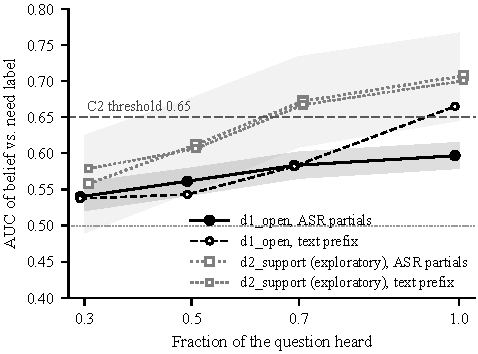
\includegraphics[width=\columnwidth]{fig_v2_prefix_auc.pdf}
\caption{Belief quality on partial transcripts (v2, test split).}
\label{fig:prefix}
\end{figure}

\subsection{Equivalence Replication (Channels Off)}\label{sec:v2-none}
% ---- P-VII.3 -----------------------------------------------------------------
% PURPOSE: replicate Prop. 1 on new data with A1--A3 enforced.
% PREDICTION: identical decisions, Ours-v2 vs B9+ (100%); utility difference
%   inside +-0.005 by TOST [PRE2 Sec. 3 secondary family].
% NUMBERS: % NOT AVAILABLE: the channels-off ("none") replication was
%   % removed from the pre-registration before the freeze because the frozen
%   % code (ddde67f) does not implement it (PRE2 Sec. 3.4); Prop. 1 is
%   % verified on the v1 data instead (10,000/10,000 off-grid decisions;
%   % 11,300/11,300 for B9+ [V1T]); authors: drop this subsection
%   % (DRAFTING_GUIDE P-VII.3: DELETE) and the "channels-off control" note
%   % in Table~\ref{tab:predictions} has been updated accordingly.
\todo{P-VII.3: the channels-off replication of the equivalence.}

\subsection{Boundary Test (P1, P2, P3)}\label{sec:v2-boundary}
% ---- P-VII.4 P1 ----------------------------------------------------------------
% PURPOSE: Delta_C against B9+, with CI and one-sided p.
% NUMBERS [docs/research_v2/v2_test_results_final.json per_dataset.<ds>.primary,
%   pooled; Table~\ref{tab:v2primary}]:
%   d1_open (pre-registered): Delta_C = -0.0367 [-0.0481, -0.0252]
%   (n = 3,734), P1 p = 1.000 -> P1 FAILS; H-REV p < 1e-4 -> holds, passes
%   Holm (threshold 0.00625). The joint controller is worse than B9+.
%   d2_support (exploratory): -0.0227 [-0.0502, +0.0047] (498 items, 192
%   pair clusters), P1 p 0.944, H-REV p 0.056 (not rejected).
%   Pooled (exploratory): -0.0351 [-0.0458, -0.0245], P1 p 1.000, H-REV
%   p < 1e-4.
%   Direction at every profile x price (descriptive, d1_open ASR): Delta_C
%   between -0.0354 and -0.0456 in all 12 cells, every CI below 0
%   (Fig.~\ref{fig:twosided}); d2_support ASR (exploratory) ranges -0.0237
%   to +0.0140, every CI includes 0.
%   Dev-predicted at the primary cell [docs/research_v2/v2_predictions.json;
%   PRE2 Sec. 3.3, 3.6]: d1_open -0.0454 (SE 0.0093), d2_support -0.0093
%   (SE 0.0189), pooled -0.0409 (SE 0.0085); predicted verdicts P1 fails,
%   H-REV likely holds -- both confirmed.
%   Mechanism on dev (PRE2 Sec. 3.6, lab log 2026-10-16): Ours-v2 retrieves
%   on 99% of d1 ASR turns and dispatches earlier than B9+, on partial
%   queries that retrieve worse (accuracy 0.438 vs 0.500) -- dev only.
%   Text-only secondary condition (text150, d1_open, primary price):
%   Delta_C = -0.0024 [-0.0072, +0.0022], a tie (descriptive)
%   [v2_test_results_d1.md] -- the gap is an ASR-partial effect.
\todo{P-VII.4: P1, the commit-architecture contrast.}

% ---- P-VII.5 P2 ----------------------------------------------------------------
% PURPOSE: the paired interaction Delta_C - Delta_S on the same items; this is
%   the boundary itself.
% NUMBERS [v2_test_results_final.json; same records, both architectures,
%   same bootstrap resamples]:
%   d1_open (pre-registered): interaction Delta_C - Delta_S = +0.0047
%   [+0.0007, +0.0088], P2 one-sided p = 0.0097: rejects at 0.025 on its
%   own but FAILS Holm (threshold 0.00833 after H-REV). Read: the joint
%   controller's DEFICIT is 0.0047 smaller under commit than under
%   speculation -- not a joint advantage.
%   d2_support (exploratory): -0.0166 [-0.0381, +0.0044], p 0.940.
%   Pooled (exploratory): +0.0022 [-0.0020, +0.0065], p 0.160.
%   Dev-predicted (pooled): +0.0036 (SE 0.0037), "uncertain", power 0.31
%   [PRE2 Sec. 3.6, 6.1]. Realised SE of the d1_open interaction 0.0021,
%   MDE(80%) 0.0057 [paper_numbers_v2.json realised_precision].
\todo{P-VII.5: P2, the interaction between architecture and controller.}

% ---- P-VII.6 P3 ----------------------------------------------------------------
% PURPOSE: TOST of Delta_S against +-m3; name D*[S] (expected: B11); report
%   the diagnostics m_prophet (vs B10) and m_C1 (vs B11) next to it, labelled
%   as two-epoch theory bounds, not tests.
% READING: if the upper side fails, the joint controller keeps a speculative
%   advantage beyond belief-gated prefetch; THEORY Sec. 6.2 names the
%   possible sources (delaying a paid prefetch across several partials; C3
%   query improvement). If the lower side fails, audit the implementation.
% NUMBERS [v2_test_results_final.json]: m3 = 0.016 (frozen; PRE2 Sec. 3.2).
%   D*[S] = B9+ (d1_open), SPEC/B10 (d2_support) -- NOT B11 as expected
%   above (on d2 dev SPEC and SPEC-theta tie exactly; frozen order picks SPEC).
%   d1_open (pre-registered): Delta_S = -0.0415 [-0.0528, -0.0302]; TOST
%   upper side p < 1e-4 (rejects), lower side p = 1.000 (fails) -> P3
%   FAILS on the LOWER side: Ours-v2[S] is worse than D*[S] by more than
%   m3. Per PRE2 Sec. 3.5 this is reported, the unit tests at the frozen
%   commit are re-run, and the frozen code is not changed.
%   d2_support (exploratory): -0.0061 [-0.0380, +0.0255]; upper p 0.086,
%   lower p 0.259 -> fails (CI wider than +-m3).
%   Pooled (exploratory): -0.0373 [-0.0480, -0.0267]; upper p < 1e-4,
%   lower p 0.9998 -> fails.
%   Conjunction (IUT P1 and P2 and P3): NOT supported on d1_open, d2_support
%   or pooled. Dev-predicted: P3 fails on the lower side (dev pooled
%   Delta_S -0.0445, SE 0.0085) -- confirmed.
%   Diagnostics (descriptive, not tests; paper_numbers_v2.json
%   primary_cell_diagnostics_test from contrasts_test.json): d1_open SPEC
%   discard rate q-hat = 0.0433, lambda_c(1 + w-bar) q-hat = 0.0022;
%   d2_support 0.0046 / 0.0002.
%   m_prophet, m_C1: % NOT AVAILABLE: the frozen evaluator never computes
%   % the two-epoch bounds m_prophet and m_C1 on dev or test (only q-hat
%   % and lambda_c(1+w-bar)q-hat); authors: drop this claim.
\todo{P-VII.6: P3, the equivalence test under speculation, with the
diagnostics, and the conjunction verdict (Table~\ref{tab:v2primary},
Fig.~\ref{fig:twosided}).}

% Table -- v2 primary results. Structure complete; every cell is \TBD until
% the frozen pre-registered analysis has run on the test split.
\begin{table}[t]
\caption{v2 Primary Tests (Test Split, Pooled over \dset{d1\_open} and
\dset{d2\_support}; Paired Cluster Bootstrap, $B=10{,}000$)}
\label{tab:v2primary}
\centering
\footnotesize
\setlength{\tabcolsep}{3pt}
\begin{tabular}{@{}p{1.55cm} p{1.5cm} p{1.4cm} p{1.4cm} p{1.2cm}@{}}
\toprule
Architecture & Contrast & Predicted & Observed $\bar D$ [95\% CI] & Verdict\\
\midrule
Commit & \OursV{} $-$ \Bplus & $>0$ & \TBD{e3v2 commit} & \TBD{}\\
Speculative & \OursV{} $-$ \Bten & $\le\lamC(1+w)$ & \TBD{e3v2 spec.} & \TBD{}\\
\bottomrule
\end{tabular}
\end{table}


% fig_v2_boundary.pdf (analysis/paper_figures_v2.py; data
%   docs/research_v2/v2_test_results_final.json "cells", primary ASR
%   condition): Delta_C (top) and Delta_S (bottom) with 95% paired cluster
%   bootstrap CIs (B = 10,000) per latency profile (FAISS, FAISS + rerank,
%   remote API) x price (dev belief quantile q = 0.5/0.65/0.8/0.9).
%   Black filled circles, solid whiskers = d1_open (pre-registered
%   analysis); grey open squares, dotted whiskers = d2_support
%   (exploratory). Grey band = +-m3 (0.016). Larger marker = primary cell.
%   Not shown (kept simple): pooled values, the interaction and the
%   dev-predicted values (all in Table~\ref{tab:v2primary} comments).
%   Only the primary cell is a test; the other cells are descriptive.
\begin{figure}[t]
\centering
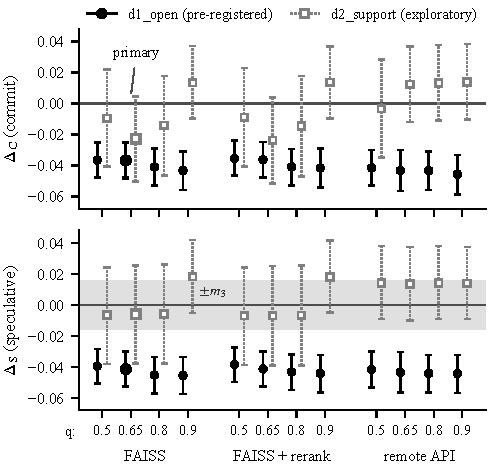
\includegraphics[width=\columnwidth]{fig_v2_boundary.pdf}
\caption{Boundary test: the joint controller's advantage over the strongest
decomposed rival under the commit ($\DC$) and speculative ($\DS$)
architectures on the same test items (v2, test split).}
\label{fig:twosided}
\end{figure}

\subsection{Secondary Analyses}\label{sec:v2-secondary}
% ---- P-VII.7 -----------------------------------------------------------------
% PURPOSE: the Holm-adjusted secondary family and the theory-fit criteria.
% CONTENT:
%   (a) architecture x dataset x profile x channel set {C1, C1+C2, C1+C2+C3}
%       with the predictions of PRE2 Sec. 3 (commit: > 0 against D*;
%       speculative: approx. 0 against D* by TOST +-m3, > 0 against B9 and
%       against B10) -- CONTRADICTS FROZEN PREREG: the channel-set cells
%       were removed before the freeze (PRE2 Sec. 3.4). The frozen
%       secondary family is 6 two-sided tests, per dataset at the primary
%       cell, Holm at 0.05 [v2_test_results_final.json secondary_family;
%       EXPLORATORY as a family because it includes d2_support]:
%       d1_open Delta_C p < 1e-4 (rejects), Delta_S p < 1e-4 (rejects),
%       interaction p 0.0194 (not rejected in the 6-test family; rejects
%       in the d1-only 3-test Holm at 0.05); d2_support Delta_C p 0.111,
%       interaction p 0.121, Delta_S p 0.717 (none rejects).
%       Descriptive cells (24 per dataset: condition x profile x price):
%       Fig.~\ref{fig:twosided} and v2_test_results_final.md "All cells";
%       text150 d1_open Delta_C at the primary price -0.0024
%       [-0.0072, +0.0022] (tie); text150 d1 range -0.0088 to +0.0013.
%   (b) C1-only cells: % NOT AVAILABLE: not run (removed before the freeze,
%       % PRE2 Sec. 3.4); authors: drop. MDE at the realised N for the
%       primary contrasts instead [paper_numbers_v2.json realised_precision;
%       MDE = 2.80 x bootstrap SE]: d1_open Delta_C 0.0165, interaction
%       0.0057; pooled 0.0153 / 0.0062 (dev prediction 0.0155 / 0.0068).
%   (c) predicted versus observed (Delta_C, dev prediction vs test)
%       [v2_test_results_final.json predicted_vs_observed_by_dataset]:
%       d1_open (pre-registered), 24 cells: Spearman 0.870 (one-sided 95%
%       lower bound 0.794), IVW slope 0.827 [0.582, 1.077] -> "agree".
%       Both datasets (48 cells; exploratory): Spearman 0.537 (lower 0.248),
%       slope 0.762 [0.524, 1.006] -> "agree". d2_support alone
%       (exploratory): Spearman 0.071, slope -0.469 -> "disagree".
%   (d) v1 frontier-dominance rule on v2: % NOT AVAILABLE: not computed --
%       % the frozen test evaluator writes only the Ours-v2 vs D* contrasts,
%       % not the per-controller accuracy / p95-TTFA operating points that
%       % analysis/e3_frontier.py needs; authors: drop this claim.
%   (e) secondary judge (GPT-4o v4) re-report of P1--P3:
%       % NOT AVAILABLE: GPT-4o graded a stratified 30% subsample of the
%       % d2_support test answers at the ANSWER level (10,330 answers), so
%       % none of the 498 items has all its cells graded by GPT-4o (median
%       % coverage 48% of an item's graded answers); a P1--P3 re-report
%       % needs a new evaluation mode not in the frozen evaluator; authors:
%       % drop the re-report. Available instead (30% subsample):
%       answer-level agreement GPT-4o vs gpt-6.1-sol on Phase A d2 test
%       answers 88.6% (n = 10,330); on E1 label draws 90.9% (n = 747)
%       [v2_test_results_final.json judge_checks; exploratory].
%   (f) waste-rate sensitivity: v1 -- B9+ = Ours on 1,300/1,300 decisions
%       at every w in {0, 0.04, 0.08, 0.16}, mean accuracy gap Ours - B9
%       +0.001 to +0.008, dominance 0/5 seeds at every w
%       [docs/research_v2/waste_sensitivity_v1.json; waste_sensitivity.md].
%       v2 d1_open (Delta_C under coef in {0, 0.04, 0.08, 0.16};
%       docs/research_v2/waste_sensitivity_v2_d1.json): [waste v2 d1: pending].
%       w itself is NOT measured in v2 (placeholder w(f) = 0.1(1 - f),
%       decision only).
%   (g) dead-air rate: % NOT AVAILABLE: no dead-air threshold was
%       % pre-registered or fixed by the authors, and the frozen test
%       % evaluator does not output per-turn TTFA per controller; authors:
%       % drop the claim (and the R1.9 promise) or state that in single-turn
%       % runs dead air equals TTFA.
\todo{P-VII.7: secondary family, theory-fit criteria, frontier dominance,
judge robustness and sensitivity analyses.}
